\documentclass{article}
\usepackage[a4paper, left=2cm, right=2cm, top=2cm, bottom=2cm]{geometry}
\usepackage[greek,english]{babel}
\usepackage[utf8]{inputenc}
\usepackage[numbers]{natbib}

\usepackage{graphicx}
\usepackage{alphabeta}
\usepackage{amsmath}
\usepackage{caption}
\usepackage{subcaption}
\usepackage{xcolor}
\usepackage{mathabx}
\usepackage{amssymb}
\usepackage{enumitem}
\usepackage{hyperref}

\captionsetup{labelformat=empty}
\subcaptionsetup{labelformat=empty}

\title{\textbf{Προσαρμοστικός Έλεγχος - Εργασία 2: Ο κανόνας MIT}}
\author{\textbf{Ονοματεπώνυμο}: Βραχωρίτη Αλεξάνδρα (A.M.: 1092793)}
\date{1 Δεκεμβρίου 2025}

\begin{document}
\maketitle
\section{Άσκηση 1η}
Μας δίνεται η συνάρτηση μεταφοράς μιας διεργασίας (plant model) ως:

\begin{equation}
    P(s) = \frac{1}{s(s+a)}
\end{equation}

\hfill\break
όπου \(a = 1\) για την ακόλουθη ανάλυση. Στόχος είναι η παρακολούθηση του μοντέλου αναφοράς (reference model)

\begin{equation}
    M(s) = \frac{\omega^2}{s^2 + 2 ζ \omega s + \omega^2}
\end{equation}

\hfill\break
με \(ζ = 0.707\) και \(ω = 2\), έχοντας ως είσοδο αναφοράς ένα σήμα \(r(t)\).

\subsection{Ο γενικός κανόνας του MIT}
Έχοντας την τετραγωνική συνάρτηση σφάλματος \(J(\theta) = \frac{1}{2}e_0^2(\theta)\), προσπαθούμε να την ελαχιστοποιήσουμε, προσδιορίζοντας την βέλτιστη τιμή της παραμέτρου \(\theta\). Για να ελαχιστοποιηθεί η τιμή της \(J\), πρέπει

\begin{equation*}
    \frac{\partial J(\theta)}{\partial \theta} = \frac{\partial}{\partial \theta}\left( \frac{1}{2} e_0^2(\theta) \right) = e_0(\theta)\,\frac{\partial e_0(\theta)}{\partial \theta} = 0.
\end{equation*}

\hfill\break
Στόχος μας είναι να οδηγήσουμε το σφάλμα \(e_0\) στο 0 και οι παράμετρος \(\theta\) να σταθεροποιηθεί, ώστε να έχουμε καλή παρακολούθηση του συστήματος. Σταθεροποίηση της παραμέτρου, σημαίνει μηδενικός ρυθμός μεταβολής της ως προς τον χρόνο, δηλαδή \(\frac{d\theta}{dt} = \dot{\theta} = 0\). Επομένως, καταλήγουμε στον κανόνα του MIT (gradient update), για τον οποίο ισχύει:  

\begin{equation*}
    \frac{d\theta}{dt} = -\gamma \cdot e_0(\theta)\,\frac{\partial e_0(\theta)}{\partial \theta}
\end{equation*}

\hfill\break
όπου \(\gamma\) ένας συντελεστής τον οποίο πρέπει να ρυθμίσουμε σωστά για να έχουμε καλή παρακολούθηση του σήματος αναφοράς και \(S = \frac{\partial e_0(\theta)}{\partial \theta}\) η συνάρτηση ευαισθησίας.

\subsection{Ο νόμος ελέγχου \(u\)} 
Η συνάρτηση μεταφοράς της διεργασίας που μας δίνεται έχει 2 πόλους \(s = 0,\,\,\,s = -a\) και κέρδος \(b = 1\), δηλαδή 3 βαθμούς ελευθερίας. Αυτό σημαίνει πως για να πετύχουμε προκαθορισμένη μεταβατική απόκριση, παρακολούθηση του μοντέλου αναφοράς και την επιθυμητή υπερύψωση, πρέπει ο ελεγκτής που θα επιλέξουμε να έχει 3 παραμέτρους. Ωστόσο, και με μόνο δύο, μπορούμε να επιτύχουμε ικανοποιητική παρακολούθηση του σήματος αναφοράς, ρυθμίζοντας κατάλληλα τον συντελεστή \(\gamma\). Επιλέγουμε, λοιπόν, τον νόμο ελέγχου:

\begin{equation*}
    u = \theta_1 \cdot r - \theta_2 \cdot y_p
\end{equation*}

\hfill\break
όπου \(\theta_1\) και \(\theta_2\) οι παράμετροι, \(r\) το σήμα αναφοράς και \(y_p\) το plant.

\subsection{Ανάλυση των μοντέλων plant και reference}
Ακολουθεί η ανάλυση του plant model, ξεκινώντας από τη συνάρτηση μεταφοράς και καταλήγοντας σε ένα σύστημα διακριτού χρόνου, βάσει του οποίου θα μοντελοποιήσουμε στην MATLAB τη συνάρτηση.
\begin{align*}
    Y_p(s) = U(s) \cdot P(s)
    & \Rightarrow Y_p(s) = (\theta_1 \cdot R(s) - \theta_2 \cdot Y_p(s)) \cdot \frac{b}{s(s+a)} \\
    & \Rightarrow Y_p(s) \cdot s(s+a) = b \cdot (\theta_1 \cdot R(s) - \theta_2 \cdot Y_p(s)) \\
    & \Rightarrow Y_p(s) \cdot s^2 + s \cdot Y_p(s) a = b \cdot (\theta_1 \cdot R(s) - \theta_2 \cdot Y_p(s)) \\
    & \Rightarrow Y_p(s) \cdot s^2 + s \cdot Y_p(s) a + b \cdot \theta_2 \cdot Y_p(s) = b \cdot \theta_1 \cdot R(s) \\
    & \Rightarrow Y_p(s) \cdot s^2 + Y_p(s) \cdot (a \cdot s + b \cdot \theta_2) = b \cdot \theta_1 \cdot R(s) \\
    & \overset{L^{-1}}{\Longrightarrow} \quad \ddot{y_p} + a \cdot \dot{y_p} + b \cdot y_p \cdot \theta_2 = b \cdot \theta_1 \cdot r \\
    & \Rightarrow \ddot{y_p} = -a \cdot \dot{y_p} - b \cdot (y_p \cdot \theta_2 - \theta_1 \cdot r) \\
    & \Rightarrow \ddot{y_p} = -a \cdot \dot{y_p} + b \cdot (\theta_1 \cdot r - \theta_2 \cdot y_p) \\
    & \Rightarrow \ddot{y_p} = -a \cdot \dot{y_p} + b \cdot u
\end{align*}

\hfill\break
Με τη μέθοδο ολοκλήρωσης του Euler μπορούμε να υπολογίσουμε τα \(\dot{y_p}\) και \(y_p\):
\begin{align*}
    & \dot{y_p}_{(new)} = \dot{y_p} + \ddot{y_p} \cdot dt \\
    & {y_p}_{(new)} = y_p + \dot{y_p} \cdot dt
\end{align*}

\hfill\break
Με όμοιο τρόπο εργαζόμαστε και για το reference model, για το οποίο προκύπτουν:
\begin{align*}
    & \ddot{y_m} = -(2\zeta\omega) \cdot \dot{y_m} - (\omega^2) \cdot y_m + (\omega^2) \cdot r \\
    & \dot{y_m}_{(new)} = \dot{y_m} + \ddot{y_m} \cdot dt \\
    & {y_m}_{(new)} = y_m + \dot{y_m} \cdot dt
\end{align*}

\subsection{Ανάλυση των συναρτήσεων ευαισθησίας}
Παραπάνω ορίσαμε την συνάρτηση ευαισθησίας \(S\). Επειδή τώρα εργαζόμαστε με δύο παραμέτρους, θα έχουμε:

\hfill\break
\begin{math}
    S_1 = \frac{\partial e_0}{\partial \theta_1}
\end{math} και
\begin{math}
    S_2 = \frac{\partial e_0}{\partial \theta_2}
\end{math}

\hfill\break
και για να προχωρήσουμε, πρέπει να προσδιορίσουμε το σφάλμα \(e_0\). Έτσι, για \(e_0 = y_p - y_m\):
\begin{align*}
    & E_0 = Y_p - Y_m = (\theta_1 \cdot R(s) - \theta_2 \cdot Y_p(s)) \cdot \frac{b}{s(s+a)} - R \cdot \frac{\omega^2}{s^2 + 2 ζ \omega s + \omega^2} \\
    \Rightarrow & E_0 = \frac{\theta_1 \cdot b}{s(s+a)} R(s) - \frac{\theta_2 \cdot b}{s(s+a)} \cdot Y_p(s)) - R \cdot \frac{\omega^2}{s^2 + 2 ζ \omega s + \omega^2}
\end{align*}

\hfill\break
Με βάση τα παραπάνω έχουμε:
\begin{align*}
    & S_1 = \frac{\partial E_0}{\partial\theta_1} = \frac{b}{s(s+a)} R(s) \\
    \overset{L^{-1}}{\Longrightarrow} \quad &\ddot{S_1} = -a \cdot \dot{S_1} - \theta_2 \cdot S_1 + b \cdot r \\
    & \dot{S}_{1(\mathrm{new})} = \dot{S_1} + \ddot{S_1} \cdot dt \\
    & S_{1(\mathrm{new})} = S_1 + \dot{S_1} \cdot dt
\end{align*}

\hfill\break
και ε όμοιο τρόπο υπολογίζουμε:

\begin{align*}
    & \ddot{S_2} = -a \cdot \dot{S_2} - \theta_2 \cdot S_2 - b \cdot y_p \\
    & \dot{S}_{2(\mathrm{new})} = \dot{S_2} + \ddot{S_2} \cdot dt \\
    & S_{2(\mathrm{new})} = S_2 + \dot{S_2} \cdot dt
\end{align*}

\subsection{Gradient update και υπολογισμός των παραμέτρων}
Αφού έχουμε προσδιορίσει όλα τα παραπάνω, προχωράμε στην ανανέωση της τιμής του \(\dot{\theta}\):

\begin{equation*}
    \frac{d\theta_1}{dt} = -\gamma \cdot e_0 \cdot S_1
\end{equation*}

\begin{equation*}
    \frac{d\theta_2}{dt} = -\gamma \cdot e_0 \cdot S_2
\end{equation*}

\hfill\break
και με ολοκλήρωση Euler, έχουμε τις τιμές των παραμέτρων:

\begin{align*}
    & {\theta_1}_{(new)} = \theta_1 + \dot{\theta_1} \cdot dt \\
    & {\theta_2}_{(new)} = \theta_2 + \dot{\theta_2} \cdot dt
\end{align*}

\subsection{Διαγράμματα ευστάθειας για σήμα αναφοράς \(r = A \cdot \sin(\omega_r \cdot t)\)}
Έχοντας ημιτονοειδές σήμα αναφοράς στην είσοδο, θα εκτελέσουμε προσομοιώσεις για να μελετήσουμε την ευστάθεια του συστήματος. Επειδή νωρίτερα το διακριτοποιήσαμε, ο έλεγχος της ευστάθειας θα γίνει ως εξής: κάθε προσομοίωση θα διαρκεί \(T \,(ms)\), το χρονικό βήμα θα είναι \(dt = 0.001\,sec\) και οι σταθερές του συστήματος \(a = 1\), \(b = 1\), \(\omega = 2\) και \(\zeta = 0.707\) αντίστοιχα. Μετά τα πρώτα \(t_{window}\,ms\) κάθε προσομοίωσης θα γίνεται έλεγχος της τιμής του σφάλματος \(e_0\) και αν αυτή παραμένει \(< \epsilon\) για το υπόλοιπο της προσομοίωσης, τότε το σύστημα θα θεωρείται ευσταθές, Επίσης, ελέγχουμε τη μέγιστη τιμή του σήματος που παράγουμε, η οποία αν ξεπερνά ένα threshold, δεν είναι αποδεκτή, σύμφωνα με το εύρος πλατών που ελέγχουμε.

\subsubsection{Προσομοιώσεις για διαφορετικά \(\epsilon\)}
Εδώ θα αλλάζουμε τη συχνότητα \(\omega_r\) και το πλάτος \(A\) του ημιτόνου, καθώς και το όριο \(\epsilon\), ώστε να παρατηρήσουμε τη συμπεριφορά του συστήματος. Το \(\gamma\) είναι σταθερό και ίσο με \(1\), το \(t_{window} = 20\,ms\) ενώ ο συνολικός χρόνος προσομοίωσης είναι \(T = 100\,ms\).

\begin{figure}[h!]
    \centering
    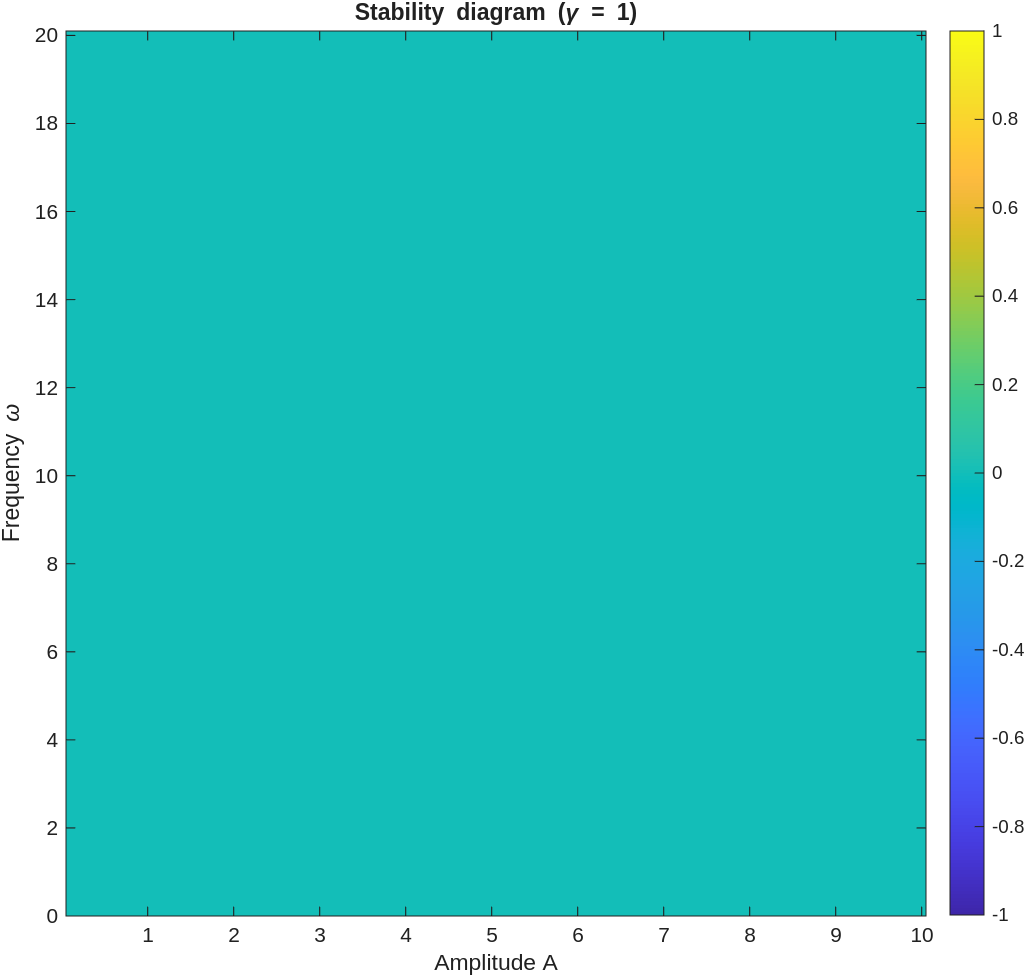
\includegraphics[width=0.65\textwidth]{1-gamma-1-T-100-tol-10e-4-3.png}
    \caption{\textbf{Διάγραμμα 1.} Το διάγραμμα ευστάθειας του συστήματος για \(\epsilon = 10^{-4}\) και \(\epsilon = 10^{-3}\).}
\end{figure}

\hfill\break
Από το Διάγραμμα ευστάθειας 1 παρατηρούμε πώς το σύστημα είναι ασταθές για οποιονδήποτε συνδυασμό πλάτους και συχνότητας στα όρια που έχουμε θέσει. Αν δοκιμάσουμε να αυξήσουμε κι άλλο το \(\epsilon\) θα εμφανίζεται περιοχή ευστάθειας στο διάγραμμα (λανθασμένα) για τιμές πλάτους \(A < 1\) και συχνότητες \(\omega_r > 6\). Η μικρή τιμή πλάτους οδηγεί σε πολύ μικρές τιμές σφάλματος \(e_0\), αλλά όχι επειδή γίνεται καλή παρακολούθηση σήματος. Άρα, τα αποτελέσματα είναι παραπλανητικά. Άλλωστε, για \(\epsilon > 10^{-3}\) δεν έχει μεγάλο φυσικό νόημα να μιλάμε για καλή παρακολούθηση, επομένως δε το μελετάμε καθόλου. 

\subsubsection{Προσομοιώσεις για διαφορετικά \(\epsilon\) και \(t_{window}\)}
Θα ακολουθήσουμε όμοια διαδικασία με πριν, αλλά για διαφορετικά παράθυρα χρόνου.

\begin{figure}[h!]
    \centering
    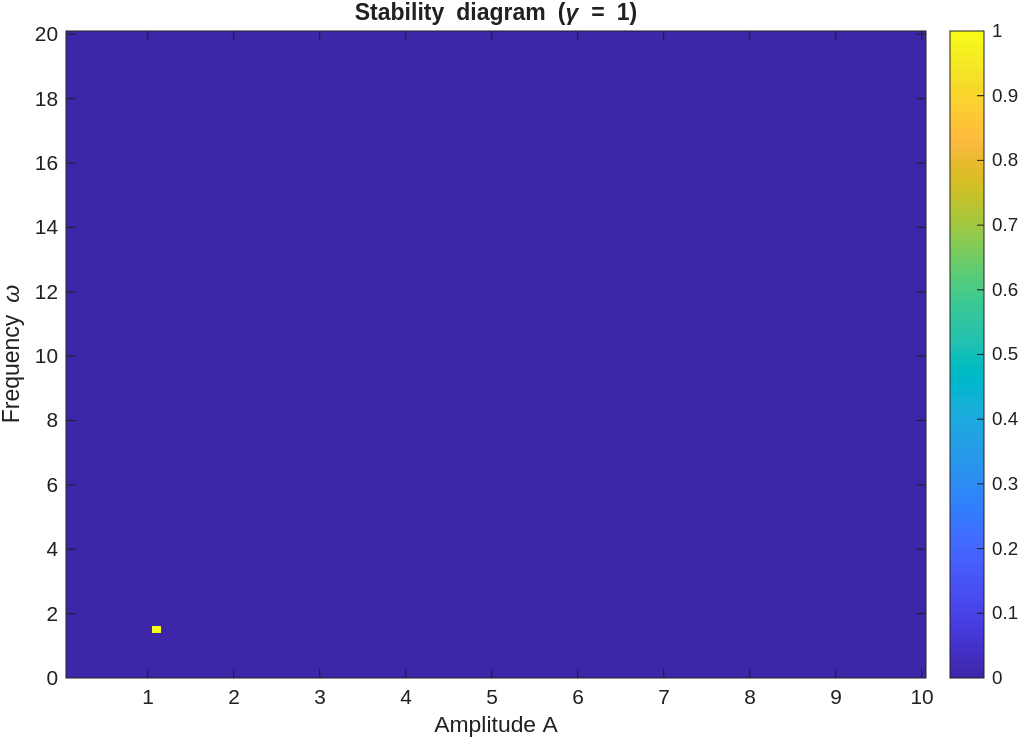
\includegraphics[width=0.7\textwidth]{1-gamma-1-T-100-tol-10e-4-tw-40.png}
    \caption{\textbf{Διάγραμμα 2.1.} Το διάγραμμα ευστάθειας του συστήματος για \(\epsilon = 10^{-4}\) και \(t_{window} = 40\).}
\end{figure}

\begin{figure}[h!]
    \centering
    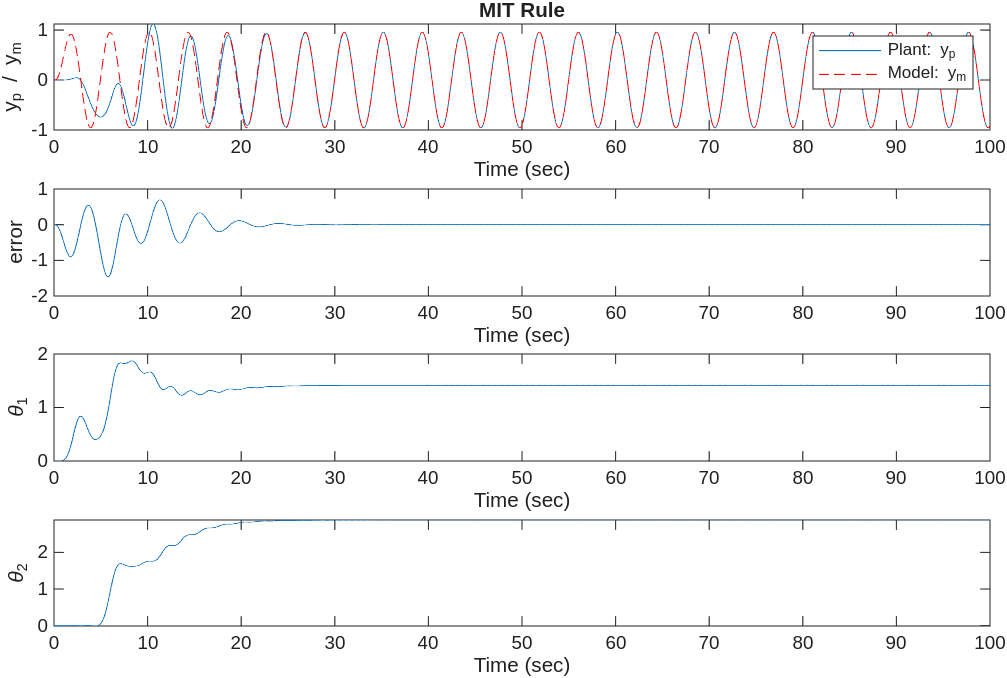
\includegraphics[width=0.7\textwidth]{1-gamma-1-T-100-tol-10e-4-tw-40-graph.png}
    \caption{\textbf{Διάγραμμα 2.2.} Αποτελέσματα προσομοίωσης για σήμα αναφοράς \(r(t) = 1.1 \cdot \sin(1.5071 t)\).}
\end{figure}

\hfill\break
Από το Διάγραμμα ευστάθειας 2.1 παρατηρούμε πώς το σύστημα είναι ευσταθές για έναν μόνο συνδυασμό πλάτους και συχνότητας, όπου \(A = 1.1\) και \(\omega_r = 1.5071\). Πράγματι, μετά τα \(40\,ms\) επιτυγχάνεται καλή παρακολούθηση. Ας εξετάσουμε όμως και μία ακόμη περίπτωση, αυξάνοντας κι άλλο το χρονικό παράθυρο, ώστε να παρατηρήσουμε τη συμπεριφορά του συστήματος.



\hfill\break
Από το  Διάγραμμα 3.1 παρατηρούμε πώς το σύστημα είναι ευσταθές για περισσότερους από έναν συνδυασμούς πλάτους και συχνότητας. Αυξάνοντας το \(\epsilon\) στο \(10^{-3}\) και διατηρώντας το \(t_{window} = 50\) βλέπουμε πώς το σύστημα είναι ευσταθές για περισσότερους συνδυασμούς πλάτους και συχνότητας σε σχέση με την περίπτωση όπου \(\epsilon = 10^{-4}\), το οποίο είναι λογικό, γιατί χαλαρώσαμε τον περιορισμό. Μπορούμε να συνεχίσουμε κάνοντας διάφορους συνδυασμούς και καταγράφοντας τη συμπεριφορά του συστήματός μας. Εδώ εξετάσαμε οριακές περιπτώσεις, εκεί που το σύστημα βρίσκεται στην πλήρη αστάθεια, έπειτα περνά σε ευστάθεια για συγκεκριμένες περιπτώσεις, οι οποίες αυξάνονται ανάλογα με τις επιλογές που κάνουμε στις προδιαγραφές μας. 

\subsubsection{Προσομοιώσεις για διαφορετικά \(\gamma\)}
Τώρα, θα διατηρήσουμε σταθερά τα \(\epsilon = 10^{-3}\), \(t_{window} = 40\,sec\) και \(T = 100\,sec\), αλλάζοντας τον συντελεστή \(\gamma\). Βρέθηκε ότι για \(\gamma < 4.5\), και για δοκιμές με βήμα \(d\gamma = 0.1\), το σύστημα δεν είναι πουθενά ευσταθές. Για τιμές μεγαλύτερες του \(4.5\) υπάρχει πάντα μια περιοχή ευστάθειας. Ας δούμε ένα παράδειγμα.

\hfill\break
\begin{figure}[h!]
    \centering
    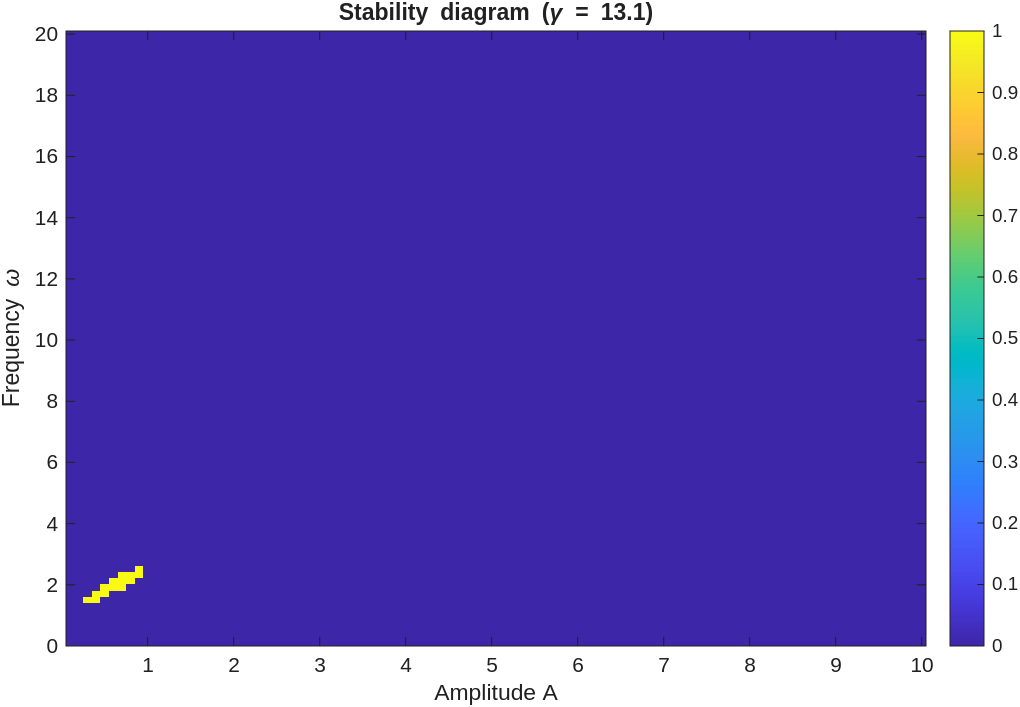
\includegraphics[width=0.8\textwidth]{1-gamma-13-1-T-100-tol-10e-3-tw-40.png}
    \caption{\textbf{Διάγραμμα 4.1.} Το διάγραμμα ευστάθειας του συστήματος για \(\gamma = 13.1\).}
\end{figure}

\begin{figure}[t]
    \centering
    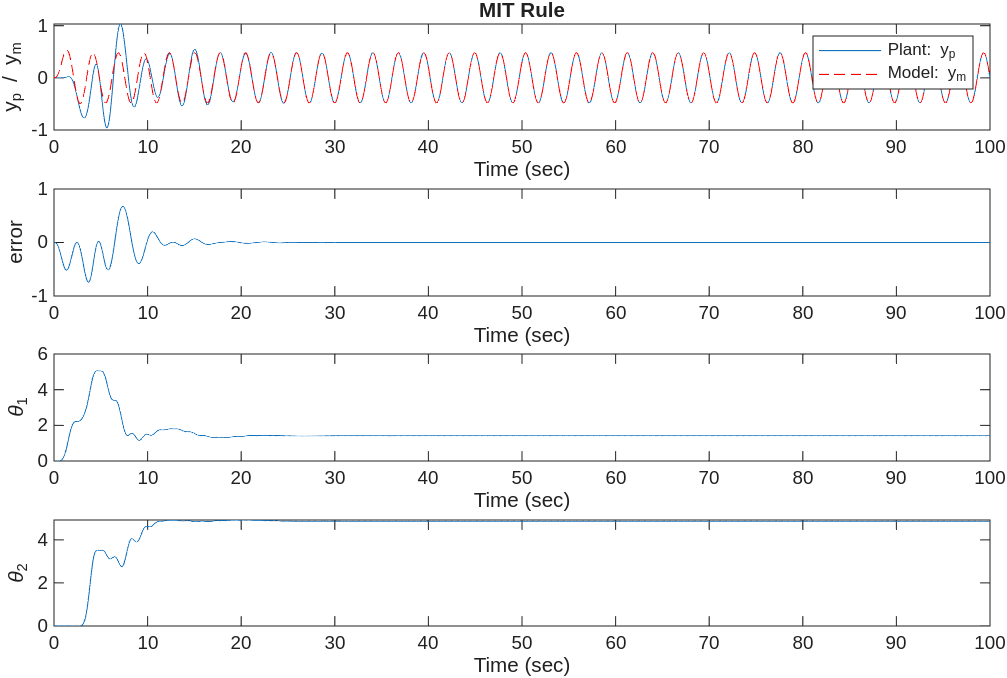
\includegraphics[width=0.8\textwidth]{1-gamma-13-1-T-100-tol-10e-3-tw-40-graph.png}
    \caption{\textbf{Διάγραμμα 4.2.} Αποτελέσματα προσομοίωσης για \(\gamma = 13.1\) και σήμα αναφοράς \(r(t) = 0.8 \cdot \sin(2.3111 t)\).}
\end{figure}

\hfill\break
\hfill\break
Αυτό που συμπεραίνουμε για την παραπάνω διαδικασία είναι ότι ο χρόνος απόκρισης του συστήματος είναι μεγαλύτερος των \(\approx 30\,sec\), ώστε το σφάλμα να παραμένει \(< \epsilon = 10^{-3}\). Όσο μικρότερο θέλουμε να είναι στο σφάλμα και ταυτόχρονα το σύστημα να παραμένει ευσταθές, ο χρόνος απόκρισης επόσης αυξάνεται. Με κατάλληλη επιλογή \(\gamma\) πράγματι μπορούμε να ελέγξουμε το σύστημά μας και να παρακολουθούμε την είσοδο αναφοράς \(r\).

\subsection{Διαγράμματα ευστάθειας για σήμα αναφοράς \(r = A\)}
Τώρα, το σήμα αναφοράς μας θα είναι μια step function, δηλαδή ένας σταθερός παλμός. Θα ακολουθήσουμε όμοια διαδικασία με πριν και θα εξάγουμε τα συμπεράσματά μας.

\subsubsection{Προσομοιώσεις για διαφορετικά \(\epsilon\)}
Εδώ θα έχουμε: \(\gamma = 1\), \(t_{window} = 20\,ms\) και \(T = 100\,ms\). 

\subsubsection{Προσομοιώσεις για διαφορετικά \(\epsilon\) και \(t_{window}\)}
Κάνοντας προσομοιώσεις για

\begin{itemize}
    \item \(\gamma = 1\), \(T = 100\,ms\), \(t_{window} = 30\,ms\) και \(\epsilon = 10^{-4}\) και
    \item \(\gamma = 1\), \(T = 100\,ms\), \(t_{window} = 30\,ms\) και \(\epsilon = 10^{-3}\)
\end{itemize}

\hfill\break
δεν υπάρχει καμία περίπτωση όπου το σύστημα είναι ευσταθές. Όμως, για \(\gamma = 1\), \(T = 100\,ms\), \(t_{window} = 30\,ms\) και \(\epsilon = 10^{-2}\) έχουμε ευστάθεια για μία τιμή πλάτους, κάτι που φαίνεται στα Διαγράμματα 5.1 και 5.2. Αυξάνοντας κι άλλο το χρονικό παράθυρο, μπορούμε να παρατηρήσουμε ότι ολοένα και περισσότερες συναρτήσεις μπορεί να τις παρακολουθήσει το σύστημά μας, αρκεί \(\epsilon = 10^{-2}\), το οποίο δεν είναι ιδιαίτερα καλό.

\begin{figure}[h!]
    \centering
    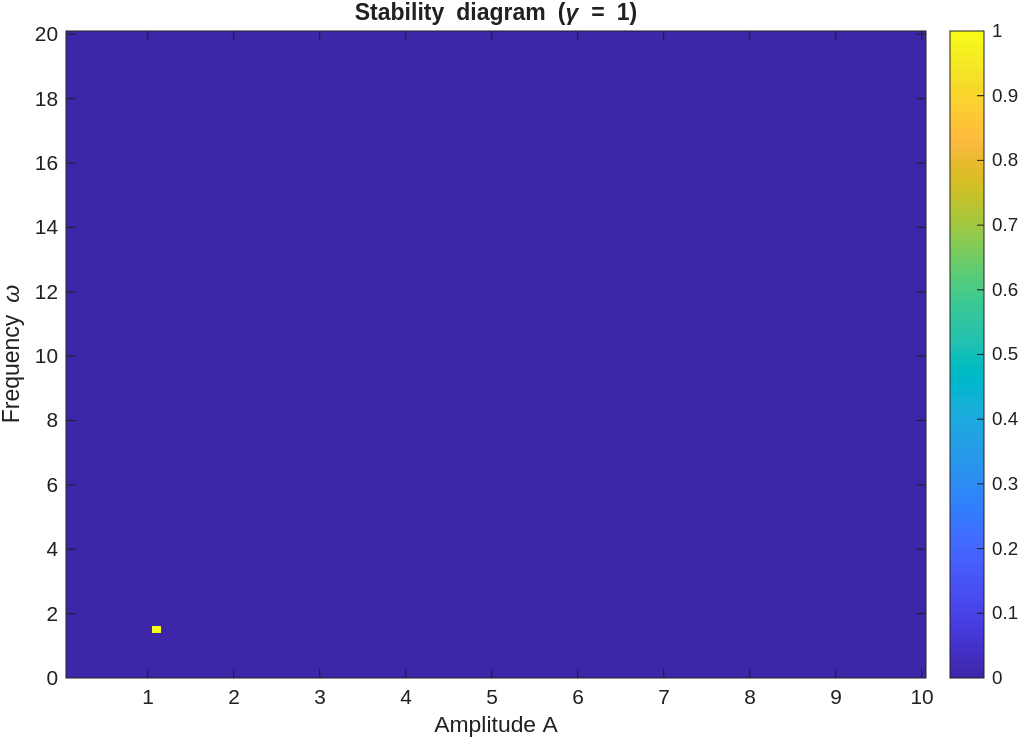
\includegraphics[width=0.7\textwidth]{1-gamma-1-T-100-tol-10e-4-tw-40.png}
    \caption{\textbf{Διάγραμμα 5.1.} Το διάγραμμα ευστάθειας του συστήματος για \(\epsilon = 10^{-2}\) και \(t_{window} = 30\).}
\end{figure}

\begin{figure}[h!]
    \centering
    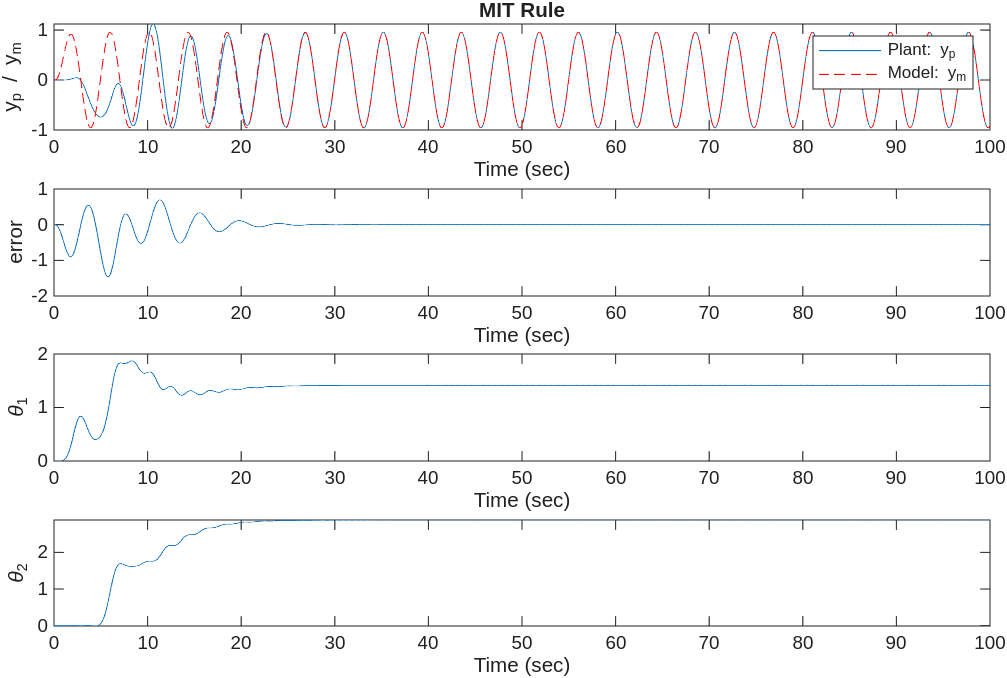
\includegraphics[width=0.7\textwidth]{1-gamma-1-T-100-tol-10e-4-tw-40-graph.png}
    \caption{\textbf{Διάγραμμα 5.2.} Αποτελέσματα προσομοίωσης για \(\epsilon = 10^{-2}\) και \(t_{window} = 30\), με σήμα αναφοράς \(r(t) = 0.4\).}
\end{figure}

\subsubsection{Προσομοιώσεις για διαφορετικά \(\gamma\)}
Τώρα, θα διατηρήσουμε σταθερά τα \(\epsilon = 10^{-3}\), \(t_{window} = 40\,sec\) και \(T = 100\,sec\), αλλάζοντας τον συντελεστή \(\gamma\). Ωστόσο, αντί να δημιουργήσουμε τα διαγράμματα ευστάθειας όπως πριν, καλύτερα ας μελετήσουμε συγκεκριμένες step functions, βρίσκοντας με ρύθμιση το κατάλληλο \(\gamma\), ώστε να διαπιστώσουμε αν πράγματι μπορεί να γίνει παρακολούθηση του συστήματος και να εξάγουμε συμπεράσματα. Ας δούμε, λοιπόν, ένα παράδειγμα.

\begin{figure}[!t]
    \centering
    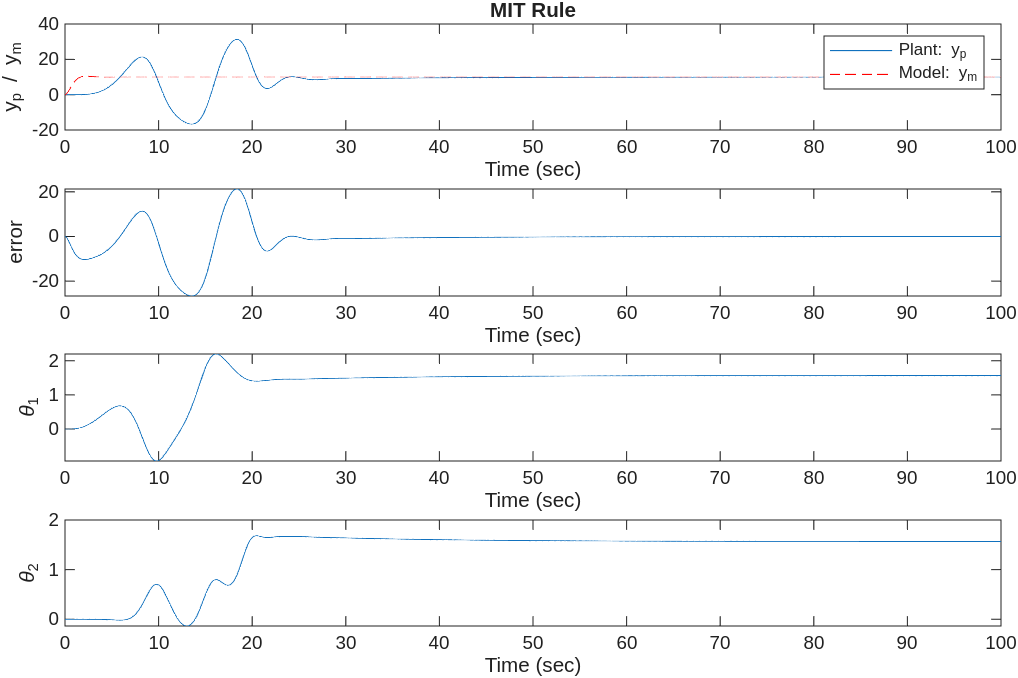
\includegraphics[width=0.8\textwidth]{1-gamma-0-0009-T-100-A-10-graph.png}
    \caption{\textbf{Διάγραμμα 6.} Αποτελέσματα προσομοίωσης για \(\gamma = 9 \cdot 10^{-4}\), με σήμα αναφοράς \(r(t) = 10\).}
\end{figure}

\hfill\break
\hfill\break
\hfill\break
Από το Διάγραμμα 6 μπορούμε να παρατηρήσουμε ότι το σφάλμα \(e_0\) πέφτει κάτω από το \(10^{-2}\) μετά τα \(90\,sec\), κάτι που κάνει το σύστημά μας εξαιρετικά αργό, σε αντίθεση με πριν, που για πολύ μικρότερο πλάτος \(A = 0.4\), το σφάλμα μειώνεται σε αυτή την τιμή μετά τα \(30\,sec\). Κάνοντας κι άλλες δοκιμές, διαπιστώνουμε ότι πράγματι, όσο το πλάτος του σήματος αναφοράς αυξάνεται, τόσο πιο πολύ καθυστερεί το σύστημα να το παρακολουθήσει.

\subsection{Παρατηρήσεις}
Θα μπορούσαμε να χρησιμοποιήσουμε σήμα ελέγχου με μία επιπλέον παράμετρο \(\theta_3\), η οποία θα μας βοηθούσε να έχουμε καλύτερη απόκριση, χωρίς τόσο μεγάλες καθυστερήσεις, μιας και όπως αναφέρθηκε, έχουμε σύστημα με 3 βαθμούς ελευθερίας.

%%%%%%%%%%%%%%%%%%%%%%%%%%%%%%%%%%%%%%%%%%%%%%%%%%%%%%%%%%%%%%%%%%%%%%%%%%%%%%%%%%%%%%%%
\hfill\break
\hfill\break
\section{Άσκηση 2η}
Μας δίνεται η συνάρτηση μεταφοράς μιας διεργασίας (plant model) ως:

\begin{equation}
    P(s) = \frac{b}{s}
\end{equation}

\hfill\break
όπου \(b = 4\). Στόχος είναι η παρακολούθηση του μοντέλου αναφοράς (reference model)

\begin{equation}
    M(s) = \frac{b_m}{s + a_m}
\end{equation}

\hfill\break
με \(a_m = 1\) και \(b_m = 2\), έχοντας ως είσοδο αναφοράς ένα σήμα \(r(t)\).

\subsection{Ανάλυση του νόμου ελέγχου, των μοντέλων και των συναρτήσεων ευαισθησίας}
Ο νόμος ελέγχου που θα χρησιμοποιήσουμε είναι όμοιος με πριν. Έτσι, για το plant model έχουμε:
\begin{align*}
    Y_p(s) = U(s) \cdot P(s)
    & \Rightarrow Y_p(s) = (\theta_1 \cdot R(s) - \theta_2 \cdot Y_p(s)) \cdot \frac{b}{s} \\
    & \Rightarrow Y_p(s) \cdot s = b \cdot (\theta_1 \cdot R(s) - \theta_2 \cdot Y_p(s)) \\
    & \overset{L^{-1}}{\Longrightarrow} \quad \dot{y_p} + b \cdot y_p \cdot \theta_2 = b \cdot \theta_1 \cdot r \\
    & \Rightarrow \dot{y_p} = b \cdot (\theta_1 \cdot r - \theta_2 \cdot y_p) \\
    & \Rightarrow \dot{y_p} = b \cdot u
\end{align*}

\hfill\break
Ξανά με τη μέθοδο ολοκλήρωσης του Euler υπολογίζουμε το \(y_p\): \begin{math} {y_p}_{(new)} = y_p + \dot{y_p} \cdot dt \end{math}

\hfill\break
Για το reference model ισχύει:
\begin{align*}
    & \dot{y_m} = -a_m \cdot y_m + b_m \cdot r \\
    & {y_m}_{(new)} = y_m + \dot{y_m} \cdot dt
\end{align*}

\hfill\break
Αντίστοιχα, για τις συναρτήσεις ευαισθησίας έχουμε:
\begin{align*}
    \begin{aligned}
        & \dot{S_1} = b \cdot (r - \theta_2 \cdot S_1) \\
        & S_{1(\mathrm{new})} = S_1 + \dot{S_1} \cdot dt
    \end{aligned}
    \qquad\qquad
    \begin{aligned}
        & \dot{S_2} = -b \cdot (\theta_2 \cdot S_2 + y_p) \\
        & S_{2(\mathrm{new})} = S_2 + \dot{S_2} \cdot dt
    \end{aligned}
\end{align*}

\subsection{Προσομοιώσεις}

\begin{figure}[h!]
    \centering
    \begin{subfigure}{0.48\textwidth}
        \centering
        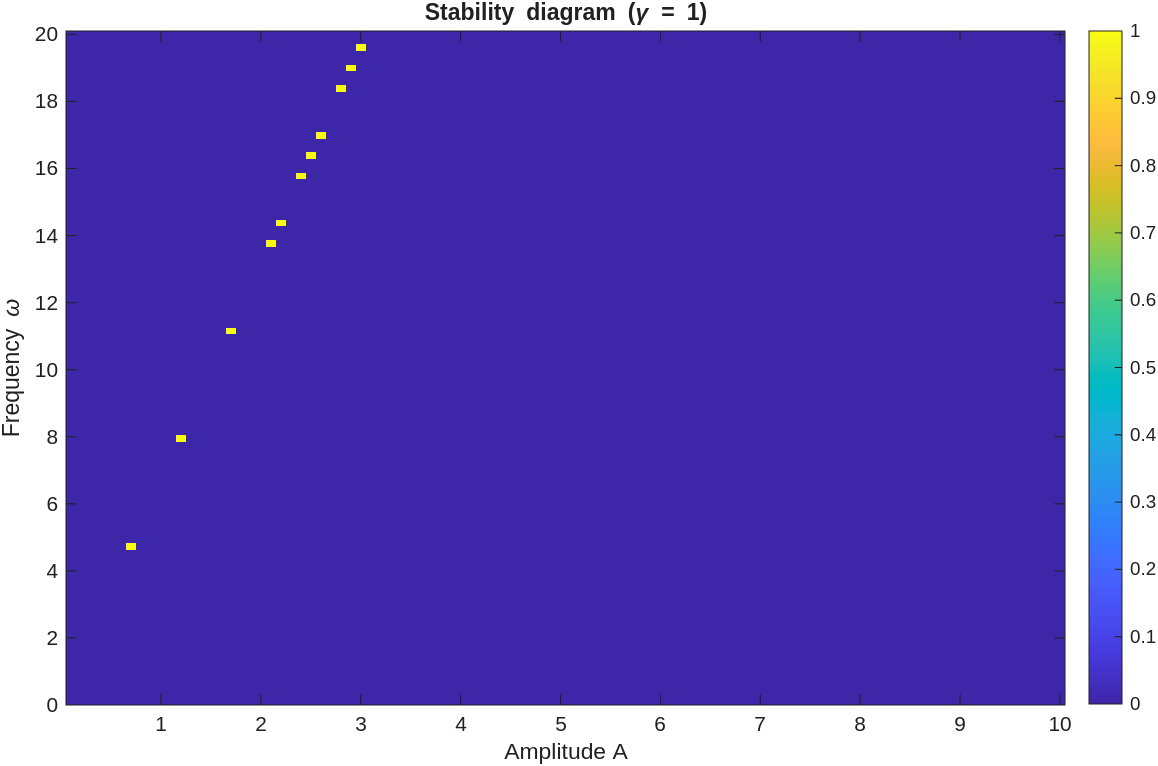
\includegraphics[width=0.8\textwidth]{2-gamma-1-T-100-tol-10e-4-tol-tw-40.png}
        \caption{\textbf{Διάγραμμα 7.1.} Το διάγραμμα ευστάθειας του συστήματος για \(\epsilon = 10^{-4}\), \(t_{window} = 40\) και \(\gamma = 1\).}
    \end{subfigure}
    \,\,\,\,
    \begin{subfigure}{0.48\textwidth}
        \centering
        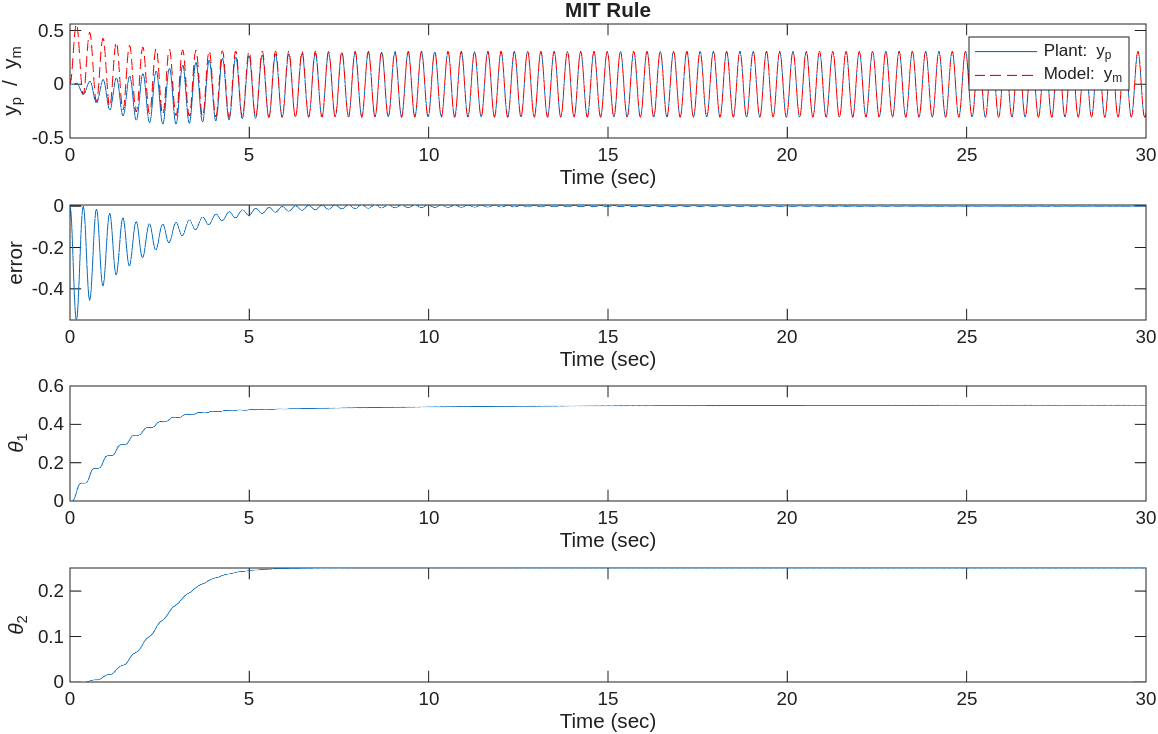
\includegraphics[width=0.8\textwidth]{2-gamma-1-T-100-tol-10e-4-tol-tw-40-graph.png}
        \caption{\textbf{Διάγραμμα 7.2.} Αποτελέσματα προσομοίωσης για το σήμα αναφοράς \(r(t) = 2.5 \cdot \sin(16.3818 t)\).}
    \end{subfigure}
\end{figure}

\hfill\break
Όπως μπορούμε να δούμε από το Διάγραμμα ευστάθειας 7.1, υπάρχουν κάποια σήματα αναφοράς για τα οποία το σύστημα είναι ευσταθές και ένα από αυτά παρουσιάζεται στο Διάγραμμα 7.2. Ωστόσο, έχει ενδιαφέρον να μελετήσουμε τη συμπεριφορά του συστήματος αν κανονικοποιήσουμε τις εξισώσεις του κανόνα MIT. Ο συντελεστής κανονικοποίησης που θα χρησιμοποιήσουμε είναι ο \(m^2(t) = 1 + S_1^2 + S_2^2\), ο οποίος εξαρτάται από τις συναρτήσεις ευαισθησίας και διαδραματίζει καθοριστικό ρόλο στο κατά πόσο οι παράμετροι του συστήματος θα αποκλίνουν ώστε να διατηρήσουν τη σταθερότητά του \cite{binh2025robust}. Αυτό μας βοηθά να αντιμετωπίσουμε έναν θεμελιώδη περιορισμό του κανόνα κανόνα MIT, όπου οι παράμετροι μπορούν να αυξηθούν απεριόριστα παρουσία διαταραχών ή σφαλμάτων 

\hfill\break
\begin{figure}[h!]
    \centering
    \begin{subfigure}{0.48\textwidth}
        \centering
        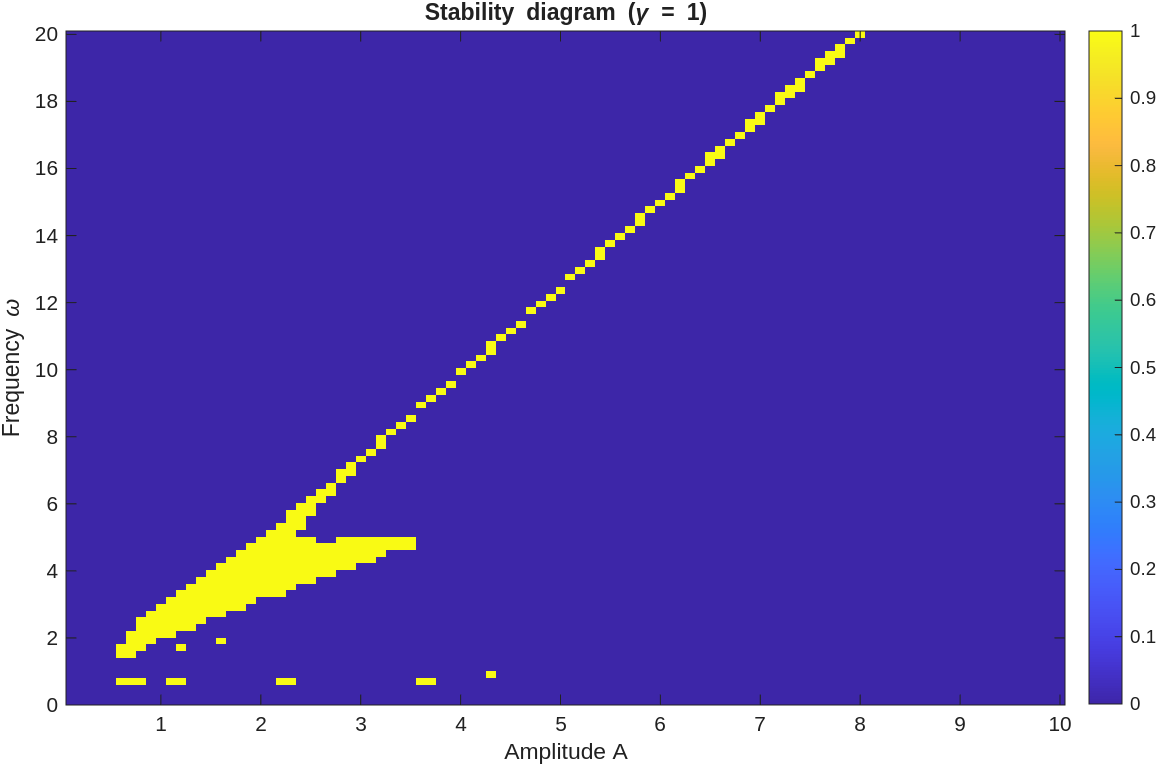
\includegraphics[width=0.8\textwidth]{2-gamma-1-T-100-tol-10e-4-tol-tw-40-norm.png}
        \caption{\textbf{Διάγραμμα 8.1.} Το διάγραμμα ευστάθειας του συστήματος για \(\epsilon = 10^{-4}\), \(t_{window} = 40\) και \(\gamma = 1\), με κανονικοποιημένο τον κανόνα MIT.}
    \end{subfigure}
    \,\,\,\,
    \begin{subfigure}{0.48\textwidth}
        \centering
        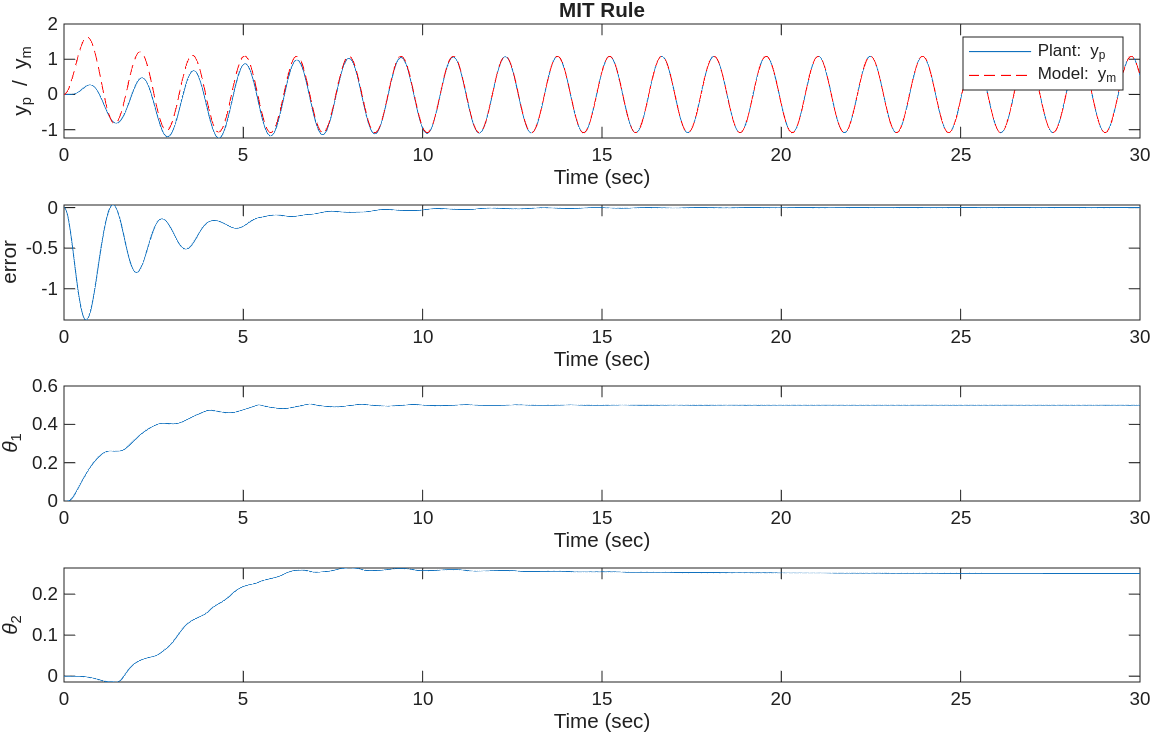
\includegraphics[width=0.8\textwidth]{2-gamma-1-T-100-tol-10e-4-tol-tw-40-norm-graph.png}
        \caption{\textbf{Διάγραμμα 8.2.} Αποτελέσματα προσομοίωσης για το σήμα αναφοράς \(r(t) = 2.4 \cdot \sin(4.3212 t)\), με κανονικοποιημένο τον κανόνα MIT.}
    \end{subfigure}
\end{figure}

\hfill\break
Εδώ είναι εμφανές ότι αυξάνεται το πλήθος των σημάτων αναφοράς για τα οποία το σύστημα παραμένει ευσταθές για ένα συγκεκριμένο \(\gamma\). Σημαντικό είναι ότι χωρίς την κανονικοποίηση, αν μειώσουμε το χρονικό παράθυρο σε \(t_{window} = 30\), το σύστημα είναι ασταθές για οποιοδήποτε σήμα αναφοράς \(r\), σε αντίθεση με την περίπτωση της κανονικοποίησης. Ας δούμε τα Διαγράμματα ευστάθειας 8.1 και 8.2.

\subsection{Παρατηρήσεις}
Παρόμοια ανάλυση μπορούμε να κάνουμε και για το σύστημα της προηγούμενης άσκησης. Εδώ, μπορούμε επιπλέον να μελετήσουμε τη συμπεριφορά του συστήματος για διαφορετικά \(\gamma\), όπου θα μας δίνουν μικρότερη ή μεγαλύτερη περιοχή ευστάθειας αντίστοιχα ή και να ρυθμίσουμε το χρονικό παράθυρο και την απόκλιση του σφάλματος, ώστε να εντοπίσουμε τα όρια του συστήματος και του κανόνα MIT.

\begin{figure}[h!]
    \centering
    \begin{subfigure}{0.48\textwidth}
        \centering
        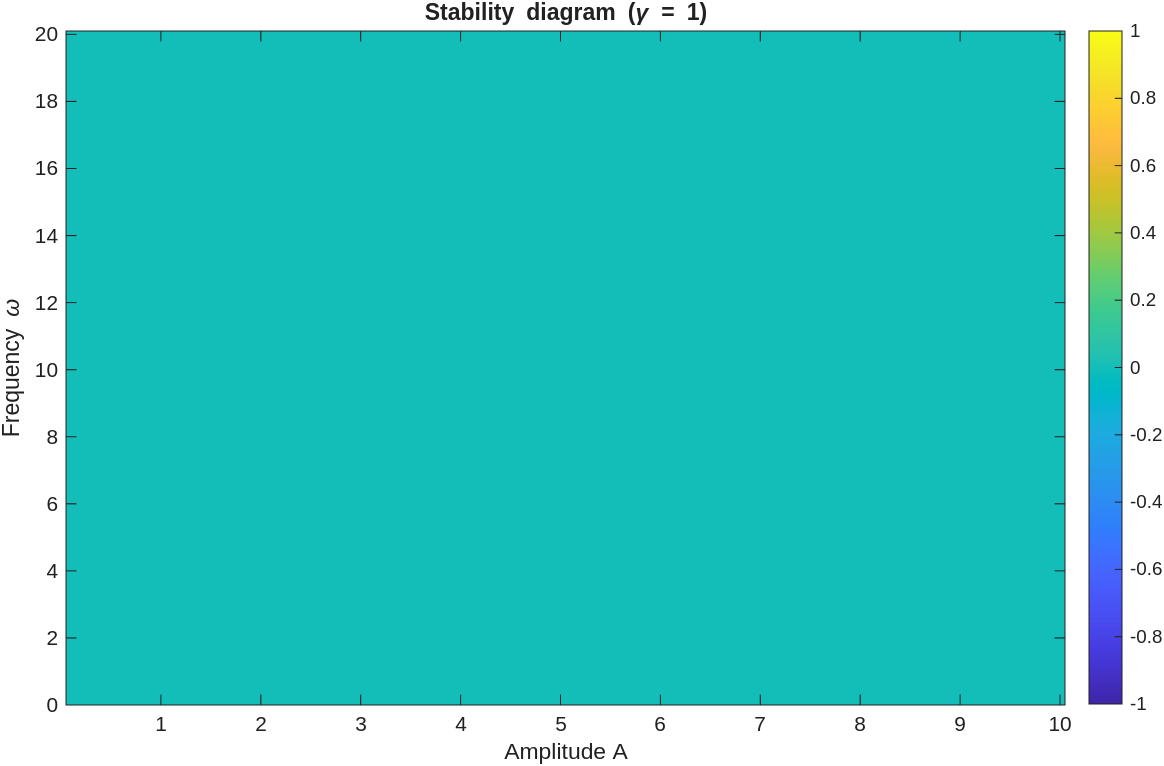
\includegraphics[width=0.8\textwidth]{2-gamma-1-T-100-tol-10e-4-tol-tw-30.png}
        \caption{\textbf{Διάγραμμα 9.1.} Το διάγραμμα ευστάθειας του συστήματος για \(\epsilon = 10^{-4}\), \(t_{window} = 30\) και \(\gamma = 1\), χωρίς κανονικοποίηση.}
    \end{subfigure}
    \,\,\,\,
    \begin{subfigure}{0.48\textwidth}
        \centering
        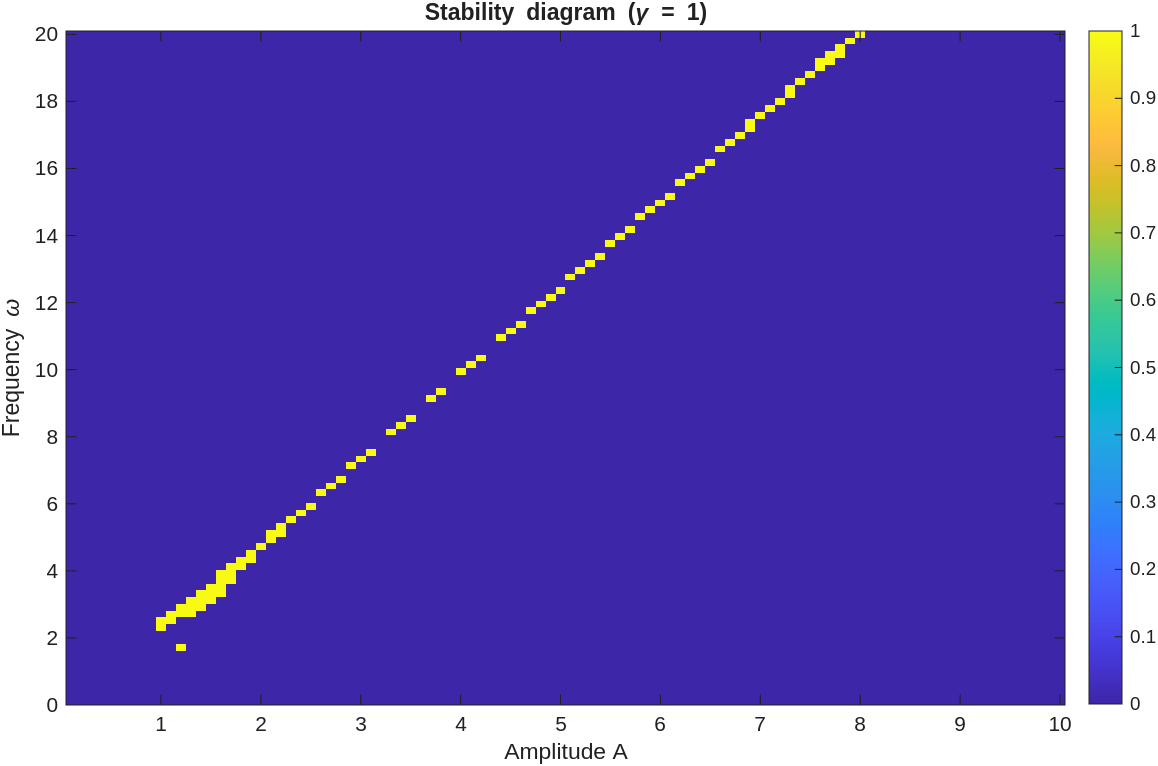
\includegraphics[width=0.8\textwidth]{2-gamma-1-T-100-tol-10e-4-tol-tw-30-norm.png}
        \caption{\textbf{Διάγραμμα 9.2.} Το διάγραμμα ευστάθειας του συστήματος για \(\epsilon = 10^{-4}\), \(t_{window} = 30\) και \(\gamma = 1\), με κανονικοποίηση.}
    \end{subfigure}
\end{figure}

\renewcommand{\refname}{Αναφορές}
\bibliographystyle{IEEEtranN}
\bibliography{references}
\end{document}